\newpage
  \section{ }%Как посчитать щели
  \label{sec:calc_slits_ability}

  Для того чтобы получить зависимость пропускной способности в зависимости от угла,
  под которым распространяется рентгеновский луч, необходимо спроецировать границы
  щелей на уровень источника.
\begin{figure}[H]
  \centering
  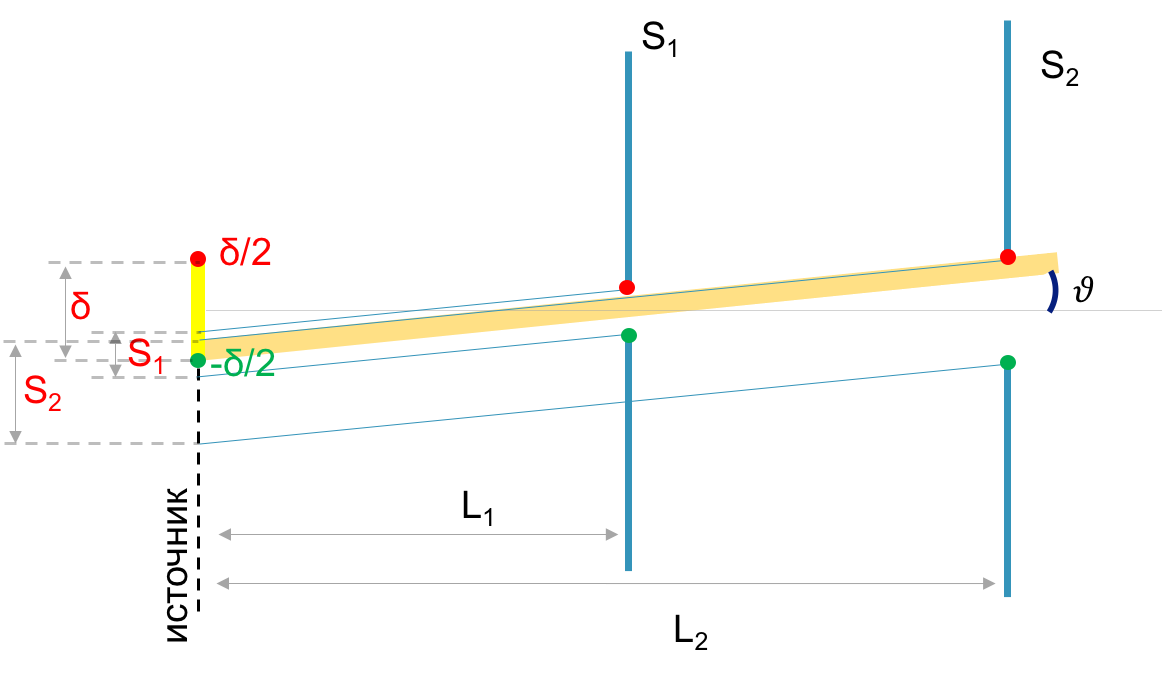
\includegraphics[width=0.6\textwidth]{images/calc_slits_ability.png}
  \caption{Для расчета пропускной способности системы щелевых коллиматоров}
  \label{ris:calc_slits_ability}
\end{figure}
$$ S^{(source)}_{1,2} = \pm \frac{S_{1,2}}{2} - \vartheta L_{1,2}.$$
 Далее находится минимальное значение проекции верхних (up):
 $$ a^{up} = min [S_1^{up,source},S_2^{up,source},\frac{\delta}{2}],$$
и максимальное значение среди проекции нижних (down):
$$ a^{down} = max [S_1^{down,source},S_2^{down,source},-\frac{\delta}{2}].$$
Следующее условие определяет величину площади параллелограмма, а соответсвенно
и характеризует пропускную способность для разных направлений $\vartheta$:
\begin{equation}
  g_s(\vartheta) =
 \begin{cases}
   0, \quad \text{если} \quad a^{down} \geq a^{up}
   \\
    (a^{up} - a^{down})L_2,\quad \text{если} \quad a^{down} < a^{up}.
 \end{cases}
\end{equation}
